% \documentclass[modern]{aastex63}
\documentclass[twocolumn]{aastex63}

\shorttitle{RR Lyrae in the Pal 5 stream}
\shortauthors{People et al.}
\newcommand{\sa}[1]{{\color{teal} SP: #1}}

% Load common packages
\usepackage{microtype}  % ALWAYS!
\usepackage{amsmath}
\usepackage{amsfonts}
\usepackage{amssymb}
\usepackage{booktabs}

\usepackage{graphicx}
\usepackage{color}

\newcommand{\documentname}{\textsl{Article}}
\newcommand{\sectionname}{Section}
\renewcommand{\figurename}{Figure}
\newcommand{\equationname}{Equation}
\renewcommand{\tablename}{Table}

% Missions
\newcommand{\project}[1]{\textsl{#1}}

% Packages / projects / programming
\newcommand{\package}[1]{\textsl{#1}}
\newcommand{\acronym}[1]{{\small{#1}}}
\newcommand{\github}{\package{GitHub}}
\newcommand{\python}{\package{Python}}
\newcommand{\emcee}{\project{emcee}}

% For referee
\newcommand{\changes}[1]{{\color{red} #1}}

% Stats / probability
\newcommand{\given}{\,|\,}
\newcommand{\norm}{\mathcal{N}}

% Maths
\newcommand{\dd}{\mathrm{d}}
\newcommand{\transpose}[1]{{#1}^{\mathsf{T}}}
\newcommand{\inverse}[1]{{#1}^{-1}}
\newcommand{\argmin}{\operatornamewithlimits{argmin}}
\newcommand{\mean}[1]{\left< #1 \right>}

% Unit shortcuts
\newcommand{\msun}{\ensuremath{\mathrm{M}_\odot}}
\newcommand{\kms}{\ensuremath{\mathrm{km}~\mathrm{s}^{-1}}}
\newcommand{\mps}{\ensuremath{\mathrm{m}~\mathrm{s}^{-1}}}
\newcommand{\pc}{\ensuremath{\mathrm{pc}}}
\newcommand{\kpc}{\ensuremath{\mathrm{kpc}}}
\newcommand{\kmskpc}{\ensuremath{\mathrm{km}~\mathrm{s}^{-1}~\mathrm{kpc}^{-1}}}

% Misc.
\newcommand{\bs}[1]{\boldsymbol{#1}}

% Astronomy
\newcommand{\DM}{{\rm DM}}
\newcommand{\feh}{\ensuremath{{[{\rm Fe}/{\rm H}]}}}
\newcommand{\df}{\acronym{DF}}
\newcommand{\logg}{\ensuremath{\log g}}
\newcommand{\Teff}{\ensuremath{T_{\textrm{eff}}}}

% TO DO
\newcommand{\todo}[1]{{\color{red} TODO: #1}}

\graphicspath{paper/}

\begin{document}

\title{Kinematics of the Palomar 5 stellar stream from RR Lyrae stars}


\author[0000-0003-0872-7098]{Adrian~M.~Price-Whelan}
\affiliation{Center for Computational Astrophysics, Flatiron Institute,
             Simons Foundation, 162 Fifth Avenue, New York, NY 10010, USA}
\affiliation{Department of Astrophysical Sciences,
             Princeton University, Princeton, NJ 08544, USA}
% \email{aprice-whelan@flatironinstitute.org}
% \correspondingauthor{Adrian M. Price-Whelan}

\author[0000-0002-6330-2394]{Cecilia~Mateu}
\affiliation{Departamento de Astronom\'ia, Facultad de Ciencias, Universidad de la Rep\'ublica, Igu\'a 4225, 14000, Montevideo, Uruguay}


\author{Giuliano~Iorio}
\affiliation{Institute of Astronomy, University of Cambridge, Madingley Road, Cambridge CB3 0HA, UK}

\author[0000-0003-0256-5446]{Sarah~Pearson}
\affiliation{Center for Computational Astrophysics, Flatiron Institute,
             Simons Foundation, 162 Fifth Avenue, New York, NY 10010, USA}

\author{Vasily~Belokurov}
\affiliation{Institute of Astronomy, University of Cambridge, Madingley Road, Cambridge CB3 0HA, UK}


\begin{abstract}
% Context
Thin stellar streams, formed from the tidal disruption of globular clusters, are important gravitational tools, sensitive to both global and small-scale properties of dark matter.
The Palomar 5 stellar stream (Pal 5) is an exemplar stream within the Milky Way: Its $\sim 20\degr$ tidal tails connect back to the progenitor cluster, and the stream has been used to study the shape, total mass, and substructure fraction of the dark matter distribution of the Galaxy.
However, most details of the phase-space distribution of the stream are not fully explained, and dynamical models that use the stream for other inferences are therefore incomplete.
% Aims
Here we aim to measure distance and kinematic properties along the Pal 5 stream in order to motivate improved models of the system. %Pal 5 stream.
We use a large catalog of RR Lyrae-type stars (RRLs) with astrometric data from the \Gaia\ mission to probabilistically identify RRLs in the Pal 5 stream.
%SP throughout the manuscript, check if you mean plural when using RRL vs RRLs.
RRLs are useful because they are intrinsically-luminous standard candles and their distances can be inferred with small relative precision ($\sim3\%$).
% Methods
% Results
By building a probabilistic model of the Pal 5 cluster and stream in proper motion and distance, we find 25 RRLs consistent with being members of the cluster (10) and stream (15).
Using these RRLs, we detect gradients in distance and proper motion along the stream, and provide an updated measurement of the distance to the Pal 5 cluster using the RRLs.
% Conclusions
We provide a catalog of Pal 5 RRLs with inferred membership probabilities for future modeling work.
\end{abstract}

\keywords{globular clusters: individual: Palomar 5 ---
stars: variables: RR Lyrae ---
Galaxy: halo ---
Galaxy: structure}

\section{Introduction} \label{sec:intro}

Globular clusters are destroyed as they orbit within the Milky Way.
The $\sim$150 bound globular clusters we presently see throughout the Galaxy \citep{Harris:2010} are therefore thought to be surviving relics of a much larger initial population, most of which were destroyed (primarily) through a combination of relaxation / evaporation and gravitational shocking from the disk and bulge \citep[e.g.,][]{Gnedin:1997, Gnedin:2014}.
As stellar systems are destroyed---i.e., as stars are tidally stripped from their progenitor---the tidal debris forms tails of matter that both lead and trail the remnant cluster, producing a stellar stream that may persist even after the progenitor is fully destroyed \citep[e.g.,][]{Johnston:1996}.

Stellar streams are useful objects because they almost \citep[see][]{Sanders:2013} delineate the past and future trajectory of their progenitor system, offering information about orbits that can be used to infer the mass distribution from the single kinematic snapshot of the Galaxy that we are afforded \citep[e.g.,][]{Johnston:1999, Sanders:2013, PriceWhelan:2014, Bonaca:2018}. % Binney:2008, Eyre:2009,
Many globular cluster stellar streams have been discovered over the last few decades \citep[see, e.g.,][]{Grillmair:2016, Shipp:2018}, in large part because of large-area, deep, multi-band imaging surveys such as the Sloan Digital Sky Survey \citep[SDSS;][]{York:2000}, Pan-STARRS PS1 survey \citep{Chambers:2016}, and Dark Energy Survey \citep{DES:2016}.
A subset of the known streams have been precisely characterized and further studied \citep[e.g.,][]{PriceWhelan:2018, Malhan:2018, Shipp:2019} using kinematic data from the recent data release 2 (\DR{2}) of the \Gaia\ mission \citep{Gaia:2016, Gaia:2018}.
Of the currently known $\sim$60 candidate stellar streams found throughout the Milky Way, few have known progenitor systems.
Conversely, of the $\sim$150 known globular clusters, only $\lesssim 20\%$ have purported tidal tails \citep[e.g.,][]{Leon:2000, Kundu:2019}, but even these are mostly low density and tenuous \citep[as might be expected, e.g.,][]{Balbinot:2018}.
%SP The above sentence makes it sound like ~<20% of the 150 known GCs have streams, is it really that many?
A prominent exception to these statements is the Palomar 5 (Pal 5) globular cluster and stream.

The Pal 5 stream---at a heliocentric distance of $d \sim 20~\kpc$---was discovered using early SDSS imaging, which reached well below the main sequence turnoff of the stream over a large area surrounding the cluster \citep{Odenkirchen:2001, Rockosi:2002}.
%SP: Maybe cite Dotter 2011 for previous distance? 
Since then, radial velocities have been measured for a handful of giant branch stars in the cluster and along the stream \citep{Odenkirchen:2002, Odenkirchen:2009, Ibata:2017}, and deeper imaging data has been used to map the tails at higher signal-to-noise \citep{Bernard:2016, Ibata:2016, Bonaca:2019}.
The detailed but still limited kinematic data for Pal 5 has made it a canonical example of tidal destruction and a useful tool for constraining Galactic structure.
For example, using the sky track and radial velocity information, the stream has been used to measure the enclosed mass of the Milky Way \citep{Kuepper:2015, Bovy:2016}.
%SP: if you say the "shape and mass", you can cite Pearson 15 too ;)
Using deep photometry, the density variations along the stream have been used to place limits on the abundance of massive substructures in the Galactic halo \citep{Erkal:2017}.

However, a number of peculiar aspects of the stream still remain unexplained in detail.
For example, the leading and trailing tails have significantly different total star counts and lengths \citep{Dehnen:2004, Bernard:2016}, and the stream track, width, and density vary significantly over the full extent of the stream \citep{Ibata:2016, Bonaca:2019}.
%SP: Might be work stating how big the estimated mass difference is in the trailing, leading vs cluster, as many people seem to be curious about this.
Given that Pal 5's pericenter is well within the Galactic disk ($r_{\textrm{peri}} \sim 7$--$8~\kpc$), 
%SP: cite erkal 2017 here (his fig 
these features could be a sign of perturbations from molecular clouds \citep[e.g.,][]{Amorisco:2016}, interaction with the Galactic bar \citep[e.g.,][]{Pearson:2017}, signatures of past dark matter subhalo encounters \citep[e.g.,][]{Erkal:2017}, or some combination of all of these effects.
Mapping the stream in all six phase-space dimensions---i.e., combining deep photometry with radial velocity, distance, and proper motion measurements---will enable and motivate improved dynamical models of the stream and more precise constraints on the Galactic mass distribution \citep[e.g.,][]{PriceWhelan:2013}.
However, at its present distance, main sequence stars are barely detected and have large astrometric uncertainties in \Gaia\ \DR{2}, and other stellar tracers (e.g., giant branch stars) are not numerous enough or precise enough distance indicators to provide useful relative distance information along the stream.
% Enter: RR Lyrae-type stars.

RR Lyrae stars (RRLs) are pulsating horizontal branch giants intrinsically more luminous than main sequence turn-off stars. Although about $\sim 10,000$ time less numerous than main sequence stars, RRLs are extremely useful probes of the Galactic halo as they are well established as standard candles; they can be observed to large distances \citep{Medina:2018,Sesar:2017c}; and are reliably identified based on their photometric variability, with little to no contamination from other types of variable stars \citep[e.g.]{Holl:2018,Drake:2017,Mateu:2012}.  Their distances can be estimated based on photometric data alone, with errors that go from $\sim8\%$ in the optical to as low as 3\% in the infrared \citep{Neeley:2017, Sesar:2017a}.

Previous studies have found RRLs in Pal5's tails: the first two were found by \citet{Vivas:2001} in the QUEST survey; and more recently \citep{Ibata:2017} found about ten new RRLs using the catalog of PS1 candidate RRLs from \citet{Hernitschek:2016}. At its current distance, Pal~5's horizontal branch is bright enough ($\G\sim17.3$) to be observed by \Gaia. Therefore, combining \Gaia~DR2 proper motions with the newer PS1 RRL catalog from \citet{Sesar:2017b} --with improved classification probabilities and light curve periods--  will allows to make precise distance and proper motion measurements along the full extent of the Pal~5 stream. Both, key ingredients for dynamical modelling of the Pal~5 stream...
%meaning we can measure kinematic properties of the full stream...
\citep{Ibata:2017} found some RRL in pal 5, but no proper motions.
This is useful for modeling...
Many stream candidates found in RRL alone \citep{Mateu:2018}.


%---yes, I rewrite things many times. C.---
%RR Lyrae stars (RRLs) are pulsating horizontal branch giants intrinsically more luminous than main sequence stars, but about $\sim 10,000$ time less numerous. At its current distance, Pal~5's horizontal branch is bright enough ($\G\sim17.3$) to be observed by \Gaia, so it's full extent can be traced and it's kinematic properties measured using RRLs. These stars can be reliably identified based on their photometric variability, with little to no contamination from other types of variable stars \citep[e.g.]{Holl2018,Drake2017,Mateu2012}, and are well known standard candles. Their distances can be estimated based on photometric data alone by means of their period-luminosity relation, with distance errors that go from $\sim8\%$ in the optical to as low as 3\% in the infrared \citep{Neeley:2017, Sesar:2017a}.  Previous studies have found RRLs in Pal5's tails: In the QUEST survey, \citet{Vivas2005} found 2 RRLs; while  \citep{Ibata:2017} found 12 RRLs using the catalog of PS1 candidate RRLs from \citet{Hernitschek2015}. Combining \Gaia~DR2 proper motions with the newer PS1 RRL catalog from \citet{Sesar2017b} --with improved classification probabilities and light curve periods--  will allow for precise distance and proper motion measurements along the full extent of the Pal~5 stream.
In this Article, we construct a probabilistic model for kinematic properties of RRLs in the vicinity of the Pal 5 stream to determine membership probabilities and thus map the distance and proper motion trends in the stream.
In \sectionname~\ref{sec:data}, we describe the source RR Lyrae catalog we use to search for Pal 5 members.
In \sectionname~\ref{sec:membership}, we implement a probabilistic membership model to identify candidate members of the stream using distance and astrometric information.
In \sectionname~\ref{sec:results}, we ...


\section{Data} \label{sec:data}

\begin{figure*}[t!]
\begin{center}
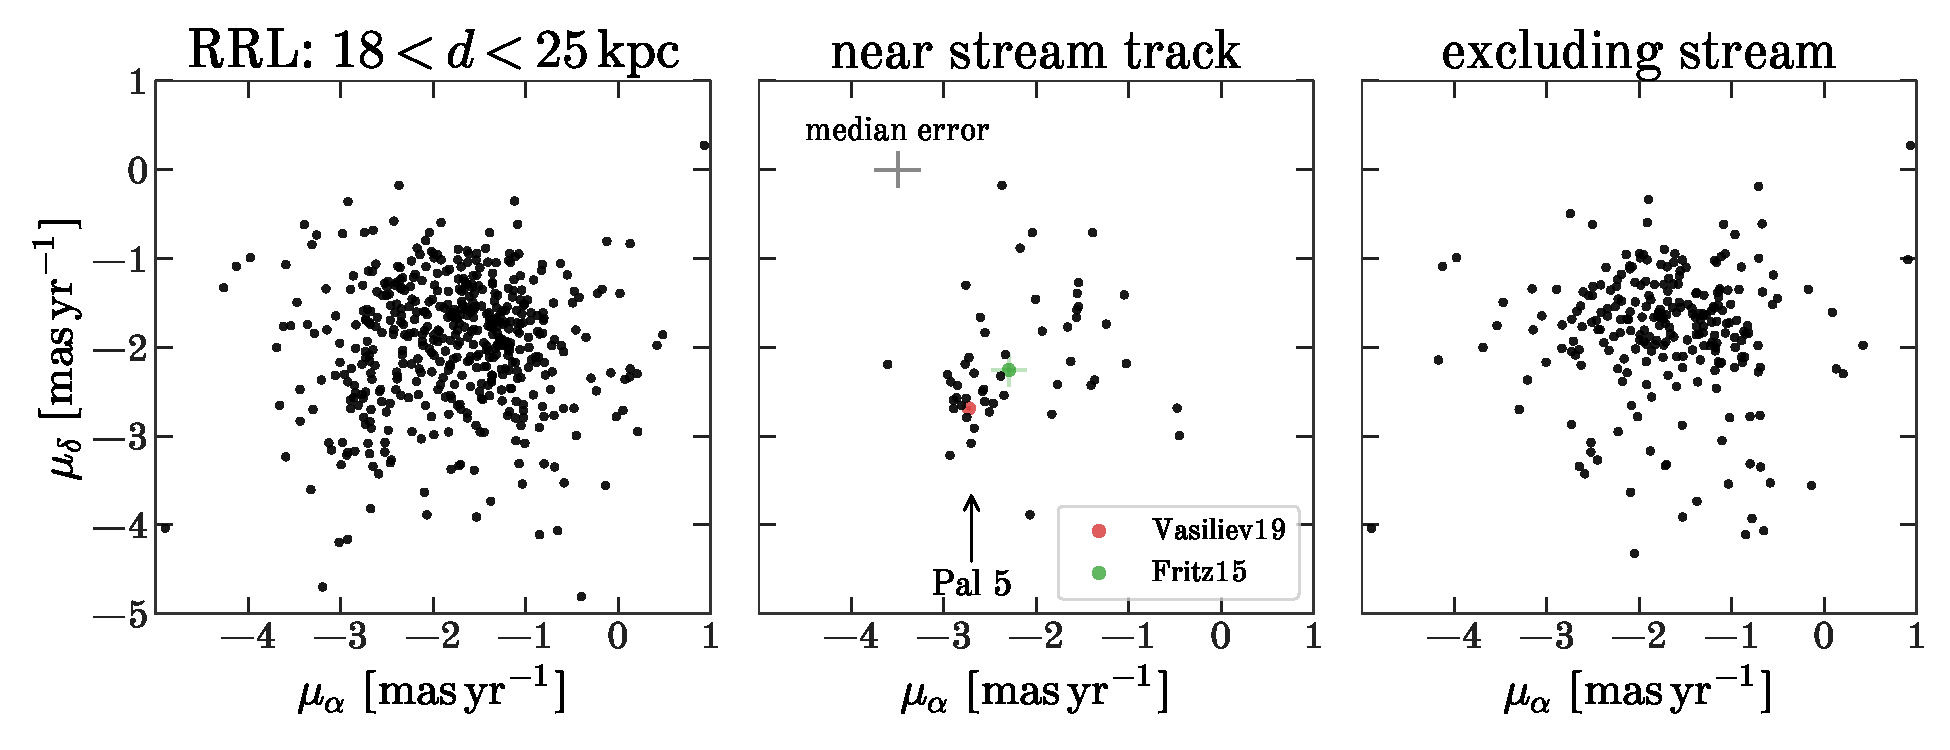
\includegraphics[width=\textwidth]{proper-motion.pdf}
\caption{\textbf{Left}: Proper motions of RRLs in the region $215^\circ < \alpha < 255^\circ$, $-15^\circ < \delta < 10^\circ$ with distances in the range $18 < d < 25~\kpc$.
\textbf{Middle}: The same, but for RRLs within $1~\degr$ of the mean sky track of Pal 5 \citep{Bonaca:2019}.
The over-density of stars near $(-2.7, -2.7)$ is the stream, and the two colored points show the Pal 5 cluster proper motions from \citet{Vasiliev:2019} and \citet{Fritz:2015}, respectively.
\textbf{Right}: The same, but for RRLs excluding $2~\degr$ around the Pal 5 sky track.}
\label{fig:pm}
\end{center}
\end{figure*}

\todo{This part was rewritten to reflect the catalog we ended up using. CM.}

The PanSTARRS-1 (PS1) catalog of RRLs \citep{Sesar:2017b} contains 229K stars spanning $\sim$3/4 of the sky (all sky north of declination $\delta > -30\degr$), with multi-epoch $grizy$ data up to a limiting magnitude $r\sim21$ (corresponding to $G \sim 21$ for the typical colors of RRLs). These stars were identified as RRLs using machine-learning methods based on a template fitting algorithm that can find pulsation periods overcoming the sparse sampling of the PS1 survey ($\sim12$ epochs per filter).  

Two all-sky RR Lyrae catalogs have also been released as part of \Gaia~\DR{2} \citep[VariClassifier and Specific Object Studies][]{Holl2018, Rimoldini2018, Clementini2018}. At present, however, these catalogs are subject to more significant and spatially-varying incompleteness in this particular area of the sky due to the \Gaia\ scanning law \citep[see][]{Rimoldini2018}.

Out of the 229K RRLs in the PS1 catalog, $\sim60$K are also reported as RRLs by \Gaia~\DR{2}, the vast majority of which (49K) are part of the subset defined by \citet{Sesar:2017b} as \emph{bona fide}. This subset is comprised of 61K RRLs above classification score thresholds set by \citet{Sesar:2017b} to ensure its high purity ($>90$\%) and completeness ($>80$\%). An extra $\sim6$K stars with lower classification scores in PS1 were also found to be RRLs by \Gaia~\DR{2} and have reported pulsation periods in the SOS catalog. Most of these RRLs have matching classifications and consistent periods in the two surveys, which increases our confidence that these are true RRLs.

For our present work, therefore, we use the superset of 68\,085 stars consisting of the 61\,795 \emph{bona fide} PS1 RRLs, plus the 6\,459 non-\emph{bona fide} PS1 stars also reported in the SOS \Gaia~\DR{2} catalog. Out of these, 68\,085 RRLs (99.8\%) have astrometric information available in \Gaia~\DR{2} and all---by construction---have photometric data and pulsation periods from PS1.

%distances---
\citet{Sesar:2017b} provide distances to the RRLs based on an $i$-band Period-Luminosity-Metallicity (PLZ) relation.
This has two key advantages when compared to optical bands: The PLZ relation in the $i$-band only weakly depends on metallicity, and the impact of dust extinction is less severe at longer wavelengths.
However, distances reported for the \rrc~stars in Table~5 of \citet{Sesar:2017b} have a systematic offset with respect to the \typeab~stars.
This offset comes from having applied the same PLZ to \typeab~and \typec~stars.
This is corrected by using the `fundamentalized' period in the PLZ relation for the \rrc~stars, which is computed as $\log{P_F} = \log P + 0.126$ \citep[following][]{Braga2016}.
In what follows, we use the $i$-band PLZ distances for the RRLs.
\citet{Sesar:2017b} estimate their overall distance precision to be 3\%, of which $\sim2$\% and $\sim1$\% correspond to systematic and random uncertainties, respectively.

We cross-match the full PS1 RRL catalog with \Gaia~DR2 \citep{Gaia:2018}, using a 3" sky separation tolerance, in order to retrieve astrometric information for these stars.
Although not all PS1 RRLs have been identified as RRLs from \Gaia\ photometry, all of the PS1 RRL are present in the main point source catalog.
\figurename~\ref{fig:pm} demonstrates that Pal 5 stream members appear in the RRL catalog: This figure shows the \Gaia\ \DR{2} proper motions for all RRLs in the sky window defined above within the distance range $18 < d < 25~\kpc$, then the same for RRLs in a tight selection around the observed stream track, and then finally the same for RRLs \emph{excluding} the stream region.

\citet{Sesar:2017b} provide an estimate of their catalog's completeness as a function of distance, at high galactic latitude, based on simulations. They estimate the mean completeness to be 92\% for \rrab~and 79\% for \rrc, up to a distance of 40~kpc, well beyond the distance of Pal~5 and its tails. At the average ratio of 3 \rrc~stars per every 10 \rrab~\citep{Layden1995}, this represents a mean completeness of 89\%. We can also produce an estimate per line of sight using the methodology described in \citet{Rybizki2018}, which requires two independent catalogs to assess the completeness of both in a probabilistic manner. Using the \Gaia~DR2 VariClassifier \citet{Holl2018,Rimoldini2018} and Specific Objects Study \citep{Clementini2018} catalogs, we find a median completeness of 92\% with a standard deviation of 16\%  with no evident spatial trend across the field of Figure~\ref{fig:members}.

% \subsection{RRL Distances}

% We assume a single intrinsic magnitude $M_G=+0.63$ for all RRLs, corresponding to the mean halo metallicity $\FeH=-1.5$ according to the calibration by \citet{Muraveva2018}, and compute distances to all stars based on their $G$-band intensity-averaged magnitudes: we use \verb+int_average_g+ for stars in VC+SOS and the intensity-averaged $g$ reported by \citet{Sesar2017b} converted to the G-band using the transformation of Eq.~XX from \citet{Evans2018}. To correct for the effect of dust extinction in the apparent magnitudes, we obtain the colour excess $E(B-V)$ for each RRL from the \citet{Schlegel1998} maps, and compute the V-band extinction as $A_V=2.742E(B-V)$ assuming an $R_V$=3.1 \citep{Schlafly2011}. Finally, the extinction is transformed to the $G$ band using the calibration from Carrasco (2018, private communication):
% \begin{equation}
% \begin{split}
% f(\Gbp-\Grp, A_V) \equiv & a + b \ (\Gbp-\Grp) + c \ (\Gbp-\Grp)^2 \\
%                          & +\ d \  A_V + e\  A_V \ (\Gbp-\Grp)
% \end{split}
% \end{equation}
% \begin{equation}
%  A_G = f(\Gbp-\Grp, A_V) \cdot A_V
% \end{equation}
% where $a=0.97883$, $b=-0.14365$, $c=0.011077$, $d=0.034842$, and $e=-0.0041448$; assuming a mean colour $BP-RP=0.7$ for RRLs.

% \todo{Describe uncertainties and justification of relative precision vs. absolute error}

\section{Determining stream membership} \label{sec:membership}

In order to search for new RRL stars in the Pal 5 stellar stream, we construct a probabilistic model of the stream and background stellar distribution (simultaneously) using proper motion $(\mu_\alpha, \mu_\delta)$ and distance $d$ data for all RRL in the sky window $215^\circ < \alpha < 255^\circ$, $-15^\circ < \delta < 10^\circ$, where $(\alpha, \delta)$ are right ascension and declination.
We \emph{do not} include the known spatial extent or morphology of the Pal 5 stream in our membership model for the stream: We instead later use the sky positions to validate the modeling procedure and selection criteria we then use to define a sample of probable Pal 5 stream RRLs.
This model ultimately enables us to compute stream membership probabilities for RRL stars in a way that fully incorporates \Gaia\ error properties, while simultaneously modeling and marginalizing over uncertainties in the background RRL distribution.

To start, we use the sky track and width of Pal 5 from \citet{Bonaca:2019} to mask out a $\sim4^\circ$-wide region around the stream---and an extrapolation of the known extent of the stream---in order to define a ``background'' region that should be devoid of Pal 5 member stars.
We use RRL stars in the background region to construct an error-deconvolved density model in the 3D space of proper motion components and distance.
We use proper motions and uncertainties from \Gaia---using the provided covariance matrix between proper motion components---and distances and uncertainties as derived above (\sectionname~\ref{sec:data}).
We use \project{extreme deconvolution} \citep[\acronym{XD};][]{Bovy:XD} to optimize the parameters of a Gaussian Mixture Model (GMM) representation of the (deconvolved) background RRL density.
We first fit the background model (with \acronym{XD}) using between $3$--$12$ mixture components and evaluate the Bayesian Information Criterion (BIC) for the optimal parameters in each case.
From this, we find that the BIC is minimized for 6 mixture components: We therefore use 6 mixture components and fix the GMM model parameters to the \acronym{XD}-optimized values and use this as our background model.
We evaluate the background likelihood of all stars in the full sky region (defined above) and refer to this as $p_{{\rm bg}, n}$ (for the $n$th star) below.

\begin{figure*}[t]
\begin{center}
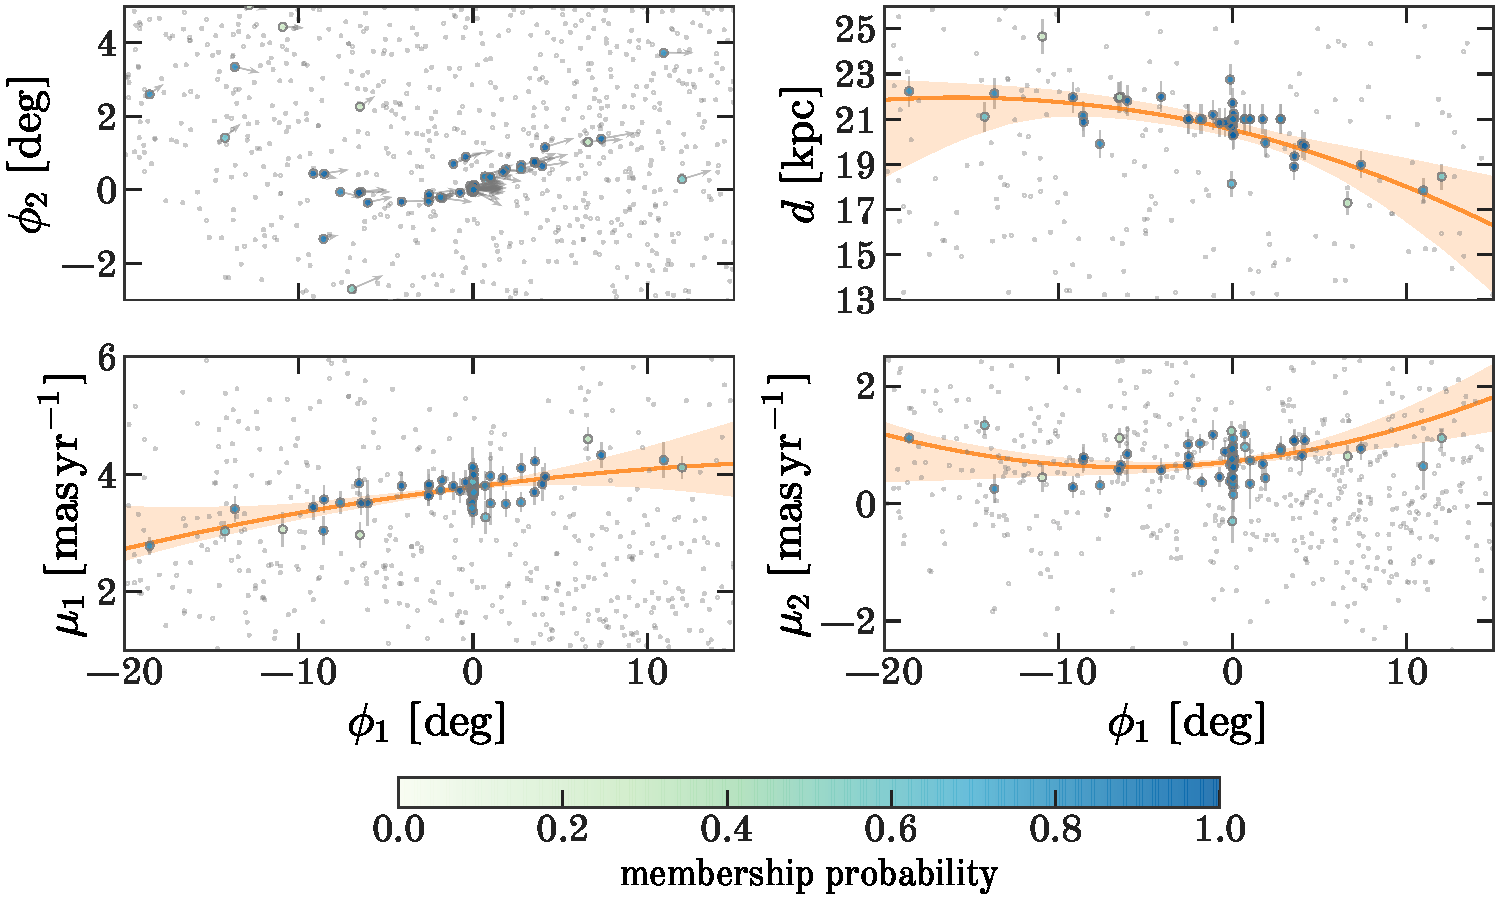
\includegraphics[width=\textwidth]{tracks.pdf}
\caption{RRL stars in the vicinity of the Pal 5 stream (with $\textrm{prob.} > 0.01$), colored by membership probability, and under-plotted with the inferred stream trends used in the membership model.
\textbf{Upper left}: Sky positions (in the Pal 5 stream coordinate frame) of RRLs, with arrows showing the \Gaia\ \DR{2} proper motion vector direction.
\textbf{Upper right}: Distance as a function of Pal 5 longitude, $\phi_1$, for the RRLs. The shaded (orange) band shows the 16--84th percentile confidence region for the inferred distance trend of the stream, and the solid line shows the median posterior sample, all assuming a quadratic function of $\phi_1$.
\textbf{Lower panels}: Same as upper right, but for the proper motion in right ascension, $\mu_\alpha$, and declination, $\mu_\delta$.
}
\label{fig:trackmembers}
\end{center}
\end{figure*}

To represent the Pal 5 stream, we use a single Gaussian component with a fixed dispersion of $0.05~\masyr$ for the proper motion components ($\approx 5~\kms$ at the distance of Pal 5) and $0.2~\kpc$ in distance.
However, we allow the mean to vary independently in each component as a function of $\phi_1$, a longitude coordinate (along the stream) as defined in \citet{Bonaca:2019}.
Based on the Pal 5 stream models from \citet{Bonaca:2019}, over the range of $\phi_1 \in (-20^\circ, 15^\circ)$, the mean stream trends in $\mu_\alpha$, $\mu_\delta$, and distance can be well-approximated (within our observational uncertainties) by a quadratic function in $\phi_1$.
The mean of our stream component, $\bs{x}$, is therefore given by
\begin{equation}
    \bs{x} = \begin{pmatrix}
        \mu_\alpha^* + b_\alpha \, \phi_1 + c_\alpha \, \phi_1^2\\
        \mu_\delta^* + b_\delta \, \phi_1 + c_\delta \, \phi_1^2\\
        d^* + b_d \, \phi_1 + c_d \, \phi_1 \label{eq:meanpoly}
    \end{pmatrix}
\end{equation}
where $\bs{\theta} = (\mu_\alpha^*, \mu_\delta^*, d^*, b_\alpha, b_\delta, b_d, c_\alpha, c_\delta, c_d)$ are free parameters.

Given the above background model, and this model for the stream track, the full likelihood for an RRL star, $n$, with data $D_n = (\mu_\alpha, \mu_\delta, d)_n$ is represented as a mixture of the two components with mixture weight $f$,
\begin{equation}
    p(D_n \given \bs{\theta}, f) = f \, \mathcal{N}(D_n \given \bs{x}, \mat{C}) + (1-f)\,p_{{\rm bg}, n}
\end{equation}
where $\mathcal{N}(\cdot \given \bs{x}, \mat{C})$ is the multivariate normal distribution with mean $\bs{x}$ and covariance matrix $\mat{C}$.

\begin{figure*}[t]
\begin{center}
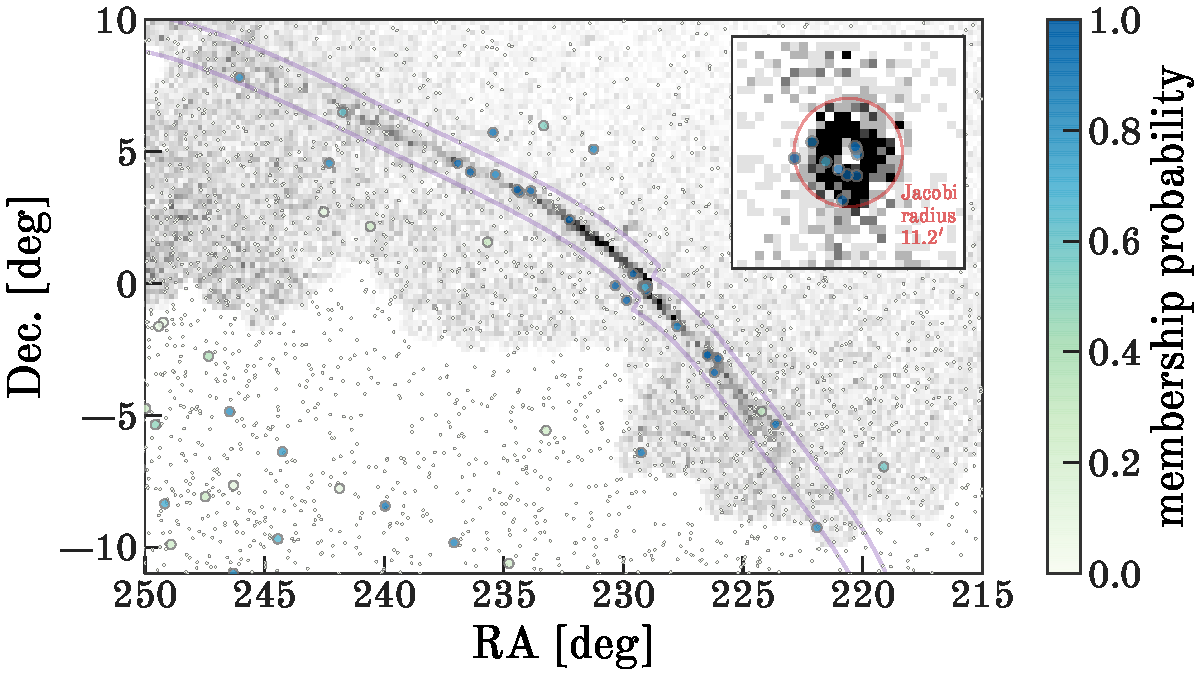
\includegraphics[width=\textwidth]{members.pdf}
\caption{Sky positions of RR Lyrae stars with Pal 5 membership probabilities $>0.01$, colored by membership probability (large markers). The background greyscale shows the surface density of CMD-filtered main sequence stars from \citet{Bonaca:2019}.}
\label{fig:members}
\end{center}
\end{figure*}

We use Markov Chain Monte Carlo (MCMC) to generate samples over the parameters $(\bs{\theta}, f)$ using the posterior probability
\begin{equation}
    p(\bs{\theta}, f \given \{D_n\}) \propto p(\bs{\theta}, f) \, \prod_n^N p(D_n \given \bs{\theta}, f)
\end{equation}
where $p(\bs{\theta}, f)$ is the prior probability distribution over the parameters.
We assume that our prior is separable in all of our parameters: We use a uniform prior for the mixture weight, $f$, such that $p(f) = \mathcal{U}(0, 1)$, Gaussian priors on the mean proper motion and distance using the Pal 5 cluster proper motion measurements from \citet{Vasiliev:2019} and the Pal 5 distance from \citet{Kuepper:2015}.
We use broad uniform priors on the linear and quadratic polynomial coefficients defined in \equationname~\ref{eq:meanpoly}.
We use the affine-invariant ensemble MCMC sampler \texttt{emcee} \citep{emcee} to sample from the posterior probability distribution given above.
We run \texttt{emcee} with 80 walkers for an initial 1024 steps to ``burn-in'' the sampler, then reset and restart the sampler for another 2048 steps.
We compute the Gelman-Rubin convergence statistic $\mathcal{R}$ \citep{Gelman:1992} to verify that $\mathcal{R} < 1.1$ for all walkers and assume that the chains have converged.
We then thin the chains by saving only every 128th step, leaving us with 1,280 posterior samples in our membership model parameters, $\bs{\theta}$.
For each star, we also compute posterior membership probabilities using the samples following \citet{DFM:blog}.

\figurename~\ref{fig:trackmembers} shows a summary of the inferred membership model properties in sky position (shown in Pal 5 coordinates $\phi_1, \phi_2$), distance, and proper motion components.
\tablename~\ref{t:rrl_members} shows an abbreviated version of our catalog of RRL in the region around Pal 5, with PS1 and \Gaia data and membership probabilities appended.

\section{Results and Discussion} \label{sec:results}

\subsection{RR Lyrae stars associated with Pal 5 and its tails}

We find a total of 24 RR Lyrae stars with membership probability $> 0.5$ that lie within $1\degr$ of the stream track \citep[again using the track from][]{Bonaca:2019}.
Of those, 13 are classified as type \typeab\ and 11 are classified as type \typec\ RRLs.
We find a total of 10 RRLs within the estimated Jacobi radius of the cluster ($\approx 12'$), meaning that 15 RRLs are spread between the leading and trailing tails.
\figurename~\ref{fig:members} shows the sky positions of all RRL with membership probability $>0.01$ over-plotted on the density of filtered main sequence stars from \citet{Bonaca:2019}.
We note that there are a few RRLs outside of the main stream track that appear to be at a consistent distance with consistent proper motions (e.g., the two stars near $\alpha = 230\degr$, $\delta = 0\degr$) that are not included in the tally above.
No theoretical models of Pal 5 have predicted tidal debris at such locations, so follow-up spectroscopy to confirm or rule out their origin would be very informative.


\subsection{Kinematics of the cluster and stream}

Past distance measurements to the Pal 5 cluster have ranged from $20.9~\kpc$ \citep{Dotter:2011} to $23.2~\kpc$ \citep{Harris:1996}, with a previous measurement from a small number of RR Lyrae stars in between at $22.3~\kpc$ \citep{Vivas:2006}.
We find a mean Pal 5 cluster distance of $20.9 \pm 0.2~\kpc$ using the PS1 RRLs and the membership model described in \sectionname~\ref{sec:membership}
This is closer than most past measurements of the cluster distance, but consistent with the measurement from \citet{Dotter:2011}.
We find a proper motion $(\mu_\alpha\,\cos\delta, \mu_\delta) = (-2.69, -2.70) \pm (0.04, 0.03)~\masyr$, consistent with the measurement in \citet{Vasiliev:2019}.
The larger proper motion (relative to \citealt{Fritz:2015} and other earlier measurements) and the closer distance means that the tangential velocity of Pal 5 is $\approx 30~\kms$ larger than most previous models have assumed.

We also detect a distance trend from the closer leading tail ($d \approx 19~\kpc$ at $\phi_1 \approx 5\degr$) to the more distant trailing tail ($d \approx 22~\kpc$ at $\phi_1 \approx -5\degr$).
While the proper motion in right ascension appears consistent with constant or only a mild gradient over the extent of the stream, we see a significant gradient in the declination component, with a difference of about $\approx 1~\masyr$ from trailing to leading tail.
% \todo{Make a table with summary information?}

\subsection{RR Lyrae population }

% Based on the prior existence of  paucity of type~\typeab\ RRL stars of in the cluster, Pal~5  would have been expected to be classified as an Oosterhoff type II cluster (ref-XX, no one really seems to say this explicitly), at odds with the cluster's known spectroscopic metallicity of $\FeH=-1.32$ \citep{TODO}, as OoII clusters are on average more metal-poor than OoI clusters.

Assuming a Jacobi radius of $12^\prime$ (computed assuming $\textrm{M}_{\rm Pal 5} \approx 1.4\times10^4~\msun$ and using the Milky Way mass model in \citealt{gala}), we find 15 RRLs in the cluster tails, 11 classified as type~\typeab\ and 4 type~\typec.
Combined with the 2 type~\typeab\ and 7 type~\typec\ RRLs in the cluster itself, there are 24 RRLs in total associated to Pal~5 and its tails with membership probabilities larger than 0.5.
In total, we find the number ratio of RRL types to be $N_{ab} / N_{c} \approx 1.2$.
\figurename~\ref{fig:PA_diagram} shows the period-amplitude diagram for the RRL stars in Pal~5.
The full sample of PS1 RRLs is shown in the background for comparison, as a grayscale density histogram. The distribution of the \typeab~RRL clearly indicate Pal~5 to be an Oosterhoff I cluster, consistent with their mean period of $0.565~d$ \todo{(XX) ?}.
Our findings of the updated ratio of \rrab~to~\rrc, mean period, and Period-Amplitude distribution of the \rrab\ RRLs all support an OoI classification for Pal~5, consistent with the cluster's metallicity, $\FeH=-1.32$ \citep{TODO}.
Out of our newly found \rrab\ RRLs, three are High Amplitude Short Period (HASP, $P <0.48$~d, $A_V>0.75$~mag $=A_g>$) stars.
This type of RRL is only found in relatively metal-rich globular clusters  \citep[$\FeH>-1.5$;][]{Monelli:2017} and the Sagittarius dwarf galaxy, but not in any other dwarf spheroidal galaxy. \todo{CM:( any other point to be made about this?)}.


\begin{figure*}[t]
\begin{center}
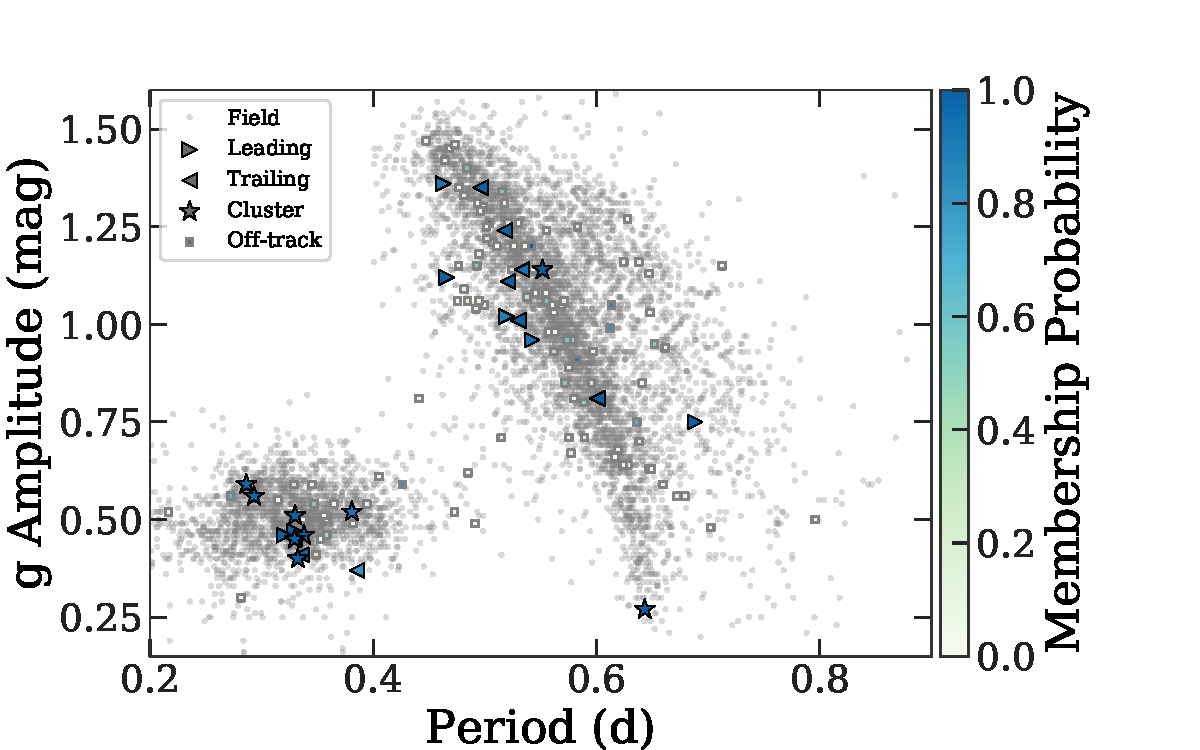
\includegraphics[width=\textwidth]{rrls_PA.pdf}
\caption{Amplitude ($g$-band) versus Period for RRLs in the Pal~5 field.}
\label{fig:PA_diagram}
\end{center}
\end{figure*}

\subsection{Stellar Mass and Luminosity}

%We can provide an estimate on the cluster's luminosity based on the observed number of RRLs. For that, the first step is to assess how complete our observed sample is.

%we obtain the completeness map shown in Figure~\ref{fig:completeness_map}, for RRLs of type \typeab~and \typec. The mean completeness estimated this way is 92\% with a standard deviation of 16\% and, as the figure shows, there is no evident spatial trend. The two estimates are remarkably consistent and, in what follows, we will adopt a completeness of 90\%-XX.

To estimate the expected absolute magnitude of Pal 5 we follow the same procedure as in \citet{Mateu:2018}, who use a linear fit of the relation between the absolute magnitude $M_V$ and the number of \typeab\ RRL, based on data from Galactic dwarf galaxies and globular clusters, here including the RR\typec~stars.  The $\log{N_{RR}}-M_V$ relation has a large scatter so, particularly for such low numbers of RRLs, it will only allow us to give rough limits on the cluster's absolute magnitude. Correcting the observed number of 26~RRLs by the median completeness of 92\%, we get a total expected number of 28~RRLs, for which we find an absolute magnitude $M_V=-8.1\pm 1.1$, which correspond to the mode and 16/84th percentiles of the posterior probability distribution.
We therefore find that the initial mass of Pal 5 \todo{...}.

% \begin{figure}
% \begin{center}
% 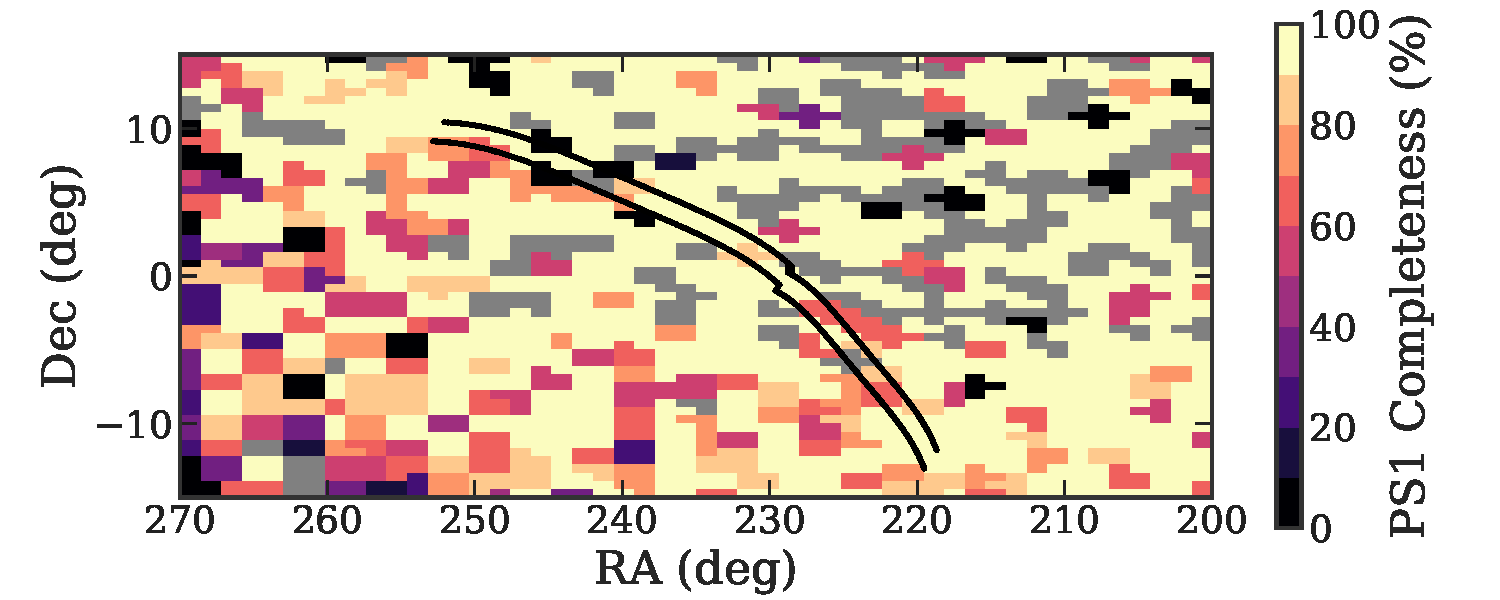
\includegraphics[width=\columnwidth]{ps1_completeness.pdf}
% \caption{PS1 RRL estimated completeness. The Pal 5 stream's track is shown with the solid line.}\label{fig:completeness_map}
% \end{center}
% \end{figure}

% \todo{CM: estimate luminosity based on number of RRLs. Compare to estimate from $M_V-\FeH$ relation. Derive stellar mass from stellar luminosity. Compare to dynamical mass estimates.}


% - there are $\sim4$-XX times as many RRLs in the tails as there are in the cluster.
% - how much mass did we already know to be in the tails compared to the cluster? (\sa{according to Ibata 2016 the mass in the present day cluster is 4297 $\pm~ 98$ M$_{\odot}$, and the streams excluding the cluster have $\sim$7903 M$_{\odot}$. So under a factor of 2 more stars in the tails than in the remnant cluster}. The cluster is thought to have had an initial mass of $\sim47000$ M$_{\odot}$). Probably not as much as a factor of 4. This makes it unexpected to have found this many RRLs in the tails. Based on prior knowledge of the mass loss undergone by the cluster we would have expected this to be XX (Sarah?/Adrian?) Similarly,


\subsection{Previously known Pal 5 RR Lyrae}

The Pal~5 cluster has 5 previous known RRL stars (named V1-V5), all of type \typec, as reported in the \citet{Clement:2001} compilation of variable stars in Galactic globular clusters and dating back to \citet{SawyerHogg:1973}.
In their analysis of the halo density profile with RRLs, \citet{Vivas:2006} report an overdensity (``Group~6'') that they claim could be associated with Pal~5's tidal tails.
% The QUEST IDs of the stars in their Group~6 are: 403, 405, 407, 411, 416 and 422.
% The first two stars --403 and 405-- are located at distances of  $9\farcm8$ and $11'$ from the cluster's center, which \citet{Vivas2004} notes places them within the cluster's tidal radius, assuming the value of $r_t\sim16'$ reported by \citet{Odenkirchen:2002}.
Two of these stars (IDs 403 and 405) are separated by just $\sim10'$ and $11'$ from the cluster's center, which places them within the cluster's Jacobi radius, and an additional star (star 393) outside of the Jacobi radius but at a similar distance could be associated with the stream \citep{Vivas:2006}.
More recently, \citet{Ibata:2017} use a prior iteration of the PS1 RRL catalog \citep{Hernitschek:2016} to identify \todo{XX} candidate members of the Pal 5 cluster and tails based on sky position and distance alone.
However, without a published catalog, we cannot compare our sample to theirs.

% In summary,  previous studies report 7 known RRLs associated to the cluster itself (1 \typeab~and 6 \typec) plus 5 more reported as possibly associated to the tails (4 \typeab~and 2 \typec).


\section{Conclusions} \label{sec:conclusions}

Using a catalog of RR Lyrae stars identified using multi-epoch, multi-band photometry from the Pan-STARRS PS1 survey and cross-matched to \Gaia\ \DR{2}, we construct a probabilistic model to determine membership with the Pal 5 cluster and stream.
We find 24 RRLs with membership probability $>0.5$ (13 type~\typeab\ and 11 type~\typec) over $\approx 18\degr$ of the stream.
From these stars, we infer the distance to the cluster, finding a closer value, $d = 20.9 \pm 0.2~\kpc$, than many past studies, and detect a distance gradient of $\sim 0.4~\kpc~{\rm deg}^{-1}$ between the trailing and leading tail (between $-5^\circ < \phi_1 < 5^\circ$).
We also, for the first time, detect trends in proper motion along the stream.
We release the full RRL catalog in the region around Pal 5 (containing distance information from PS1 and astrometry from \Gaia) with our derived membership probabilities.
These data will be instrumental for improving dynamical models of Pal 5, both for using Pal 5 to constrain the global matter distribution of the Milky Way and in interpreting the observed, complex density structure of the stream.


\acknowledgments
This work was performed in part during the Gaia19 workshop and the 2019 Santa Barbara Gaia Sprint (also supported by the Heising-Simons Foundation), both hosted by the Kavli Institute for Theoretical Physics at the University of California, Santa Barbara. The Flatiron Institute is supported by the Simons Foundation. CM acknowledges funding from the MIA program at Universidad de la Republica, Uruguay, and is grateful for the hospitality and support of the Flatiron Institute where part of this research was carried out.
This work has made use of data from the European Space Agency (ESA) mission
{\it Gaia} (\url{https://www.cosmos.esa.int/gaia}), processed by the {\it Gaia}
Data Processing and Analysis Consortium (DPAC,
\url{https://www.cosmos.esa.int/web/gaia/dpac/consortium}). Funding for the DPAC
has been provided by national institutions, in particular the institutions
participating in the {\it Gaia} Multilateral Agreement.

\software{
    Astropy \citep{astropy, astropy:2018},
    emcee \citep{emcee},
    gala \citep{gala},
    IPython \citep{ipython}
}
\clearpage
\appendix

\section{Notes on individual stars}

Star 422 is reported as an \rrc~in \citet{Vivas2004}, with a period of 0.61925~d and $V$ amplitude 0.51~mag. In PS1 it is classified as an \rrc~with a period of 0.3832276153~d. The period reported in \citet{Vivas2004} is an alias of this one, more likely to be the true period given the variability amplitude\footnote{\citet{Vivas2004} also cautions that derived periods for QUEST \rrc~stars are known to be prone to aliasing due to the observing cadence of $\sim1$~d.}. Therefore, we keep PS1's classification henceforth for RRL 422.

Star \verb+source_id=6339498589346000768+ is reported both in PS1 and \Gaia~as an \rrc~, with a period 0.4714315854~d in PS1 and 0.320110123108~d in \Gaia~SOS, the two are a pair of 1~d aliases \citep[see e.g.]{Lafler1965}. In what follows we adopt the shorter period reported in \Gaia~as the correct one as it is the more probable one for an \rrc~star.

Star \verb+source_id=4418731829516302848+ is reported in PS1 and \Gaia~as an \rrab~with a period around 0.646 and a similarly low amplitude $A_G=0.2$ and $A_g=0.3$ in both surveys. This star is reported in CRTS \citep{Drake2014} (ID CSS\_J151623.2-000831) as an \rrc~with a period 0.28164~d. We adopt the CRTS period for this star in what follows, as it is based on many more observations ($\gtrsim200$) than \Gaia~and PS1's (about a dozen per filter in each case) and the \rrc~classification and short period are more likely for such a short amplitude star.

\begin{table*}[t]
\caption{RRL members of the Pal 5 stream.}\label{t:rrl_members}
\begin{footnotesize}
\begin{tabular}{llllllll}
\toprule
\Gaia~DR2               & Other & Period & Amp-$g$ & Type & D & member & sep  \\
\verb+source_id+        & ID   & (d)    & (mag)   &     &(kpc)& prob & (") \\
\midrule
4418920808077110784 &  V5 & 0.337934& 0.46 & RRc  & 20.73 & 0.9982 &   1.9 \\
4418920846732620032 &     & 0.643239& 0.27 & RRab & 21.71 & 0.9963 &   2.0 \\
4418914863842345856 &  V1 & 0.293229& 0.56 & RRc  & 20.36 & 0.9696 &   2.0 \\
4418726027016125056 &  V3 & 0.329948& 0.51 & RRc  & 20.65 & 0.9978 &   3.8 \\
4418725889577171328 &  V4 & 0.286366& 0.59 & RRc  & 20.28 & 0.9915 &   4.5 \\
4418731829516302848 &     & 0.28164 & 0.3  & RRc  & 18.14 & 0.9297 &   4.8 \\
4418913218870688768 &  V2 & 0.332473& 0.4  & RRc  & 20.33 & 0.9977 &   5.0 \\
4418734165978521728 &     & 0.380859& 0.52 & RRc  & 22.75 & 0.9850 &   7.6 \\
4418724034151291776 & 403 & 0.551705& 1.14 & RRab & 21.23 & 0.9987 &   9.7 \\
4418732791593809152 & 405 & 0.329670& 0.45 & RRc  & 20.74 & 0.9959 &  11.0 \\
4419052204012341760 &     & 0.530006& 1.01 & RRab & 20.84 & 0.9960 &  44.5 \\
4418142117622280192 & 393 & 0.462671& 1.36 & RRab & 19.95 & 0.9060 & 118.7 \\
6339498589346000768 &     & 0.320110& 0.46 & RRc  & 18.89 & 0.9934 & 217.7 \\
6339499379619987200 &     & 0.329577& 0.47 & RRc  & 19.35 & 0.9966 & 218.6 \\
6339478312804685824 &     & 0.465883& 1.12 & RRab & 19.91 & 0.9970 & 242.8 \\
4421078432143578496 &     & 0.520749& 1.11 & RRab & 21.98 & 0.9981 & 246.1 \\
6339398155830632448 &     & 0.688316& 0.75 & RRab & 19.82 & 0.9982 & 258.9 \\
4427253907921168000 &     & 0.496334& 1.35 & RRab & 21.81 & 0.9905 & 362.5 \\
4427220338456828416 &     & 0.600796& 0.81 & RRab & 21.98 & 0.9974 & 384.4 \\
4427234700827469952 &     & 0.517911& 1.24 & RRab & 21.94 & 0.9979 & 392.3 \\
6337302795905934336 &     & 0.519462& 1.02 & RRab & 17.29 & 0.9808 & 404.5 \\
6337233350579111680 &     & 0.542383& 0.96 & RRab & 18.98 & 0.9962 & 450.6 \\
4427646704153765632 &     & 0.385552& 0.37 & RRc  & 19.90 & 0.9429 & 456.5 \\
4424705647988505600 &     & 0.335502& 0.41 & RRc  & 20.87 & 0.9832 & 513.0 \\
4426221707021159424 &     & 0.533313& 1.14 & RRab & 21.97 & 0.9728 & 550.1 \\
\bottomrule
\end{tabular}
\end{footnotesize}
\end{table*}

\bibliographystyle{aasjournal}
\bibliography{refs}

\end{document}
